% Píše: backend.
\chapter{Backend na Raspberry Pi}
\label{chap:backend}

Backend je program v~Pythonu, který na Raspberry Pi čte čidla, řídí kontrolky, světlo a~displej,
simuluje vnitřní teplotu s~termostatem a~navenek vystupuje jako periferie BLE. Formát dat, která
si program vyměňuje s~tabletem, popisuje kapitola~\ref{chap:rozhrani}.

\section{Prostředí}
\label{sec:prostredi}

Na Raspberry Pi běží Raspberry Pi OS ve vydání Trixie (64bitový, architektura aarch64)
s~Pythonem~3.13. Program je psaný pro Python od verze~3.9 a~jeho testy běží i~na PC bez
Raspberry Pi. Knihovny se instalují dvojím způsobem (tabulka~\ref{tab:knihovny}). Balíčky, které
potřebují systémové knihovny nebo se na Raspberry Pi OS dodávají předpřipravené, instaluje
skript \kod{deploy/instaluj.sh} z~apt. Ostatní instaluje pip z~\kod{requirements-pi.txt} do
virtuálního prostředí \kod{~/domek/venv}, které se vytváří s~volbou
\kod{--system-site-packages}, aby v~něm byly vidět i~knihovny z~apt.

\begin{table}[H]
\centering
\caption{Knihovny backendu}
\label{tab:knihovny}
\small
\begin{tabular}{|p{3.0cm}|p{4.2cm}|p{6.2cm}|}
\hline
\textbf{Knihovna} & \textbf{Zdroj a~verze} & \textbf{Použití} \\
\hline
bluezero & pip, \kod{bluezero==0.9.1} & periferie BLE nad rozhraním D-Bus zásobníku BlueZ \\
\hline
smbus2 & pip, bez pevné verze & sběrnice I\textsuperscript{2}C (BMP280, TSL2561) \\
\hline
RPi.bme280 & pip, bez pevné verze & kalibrace a~přepočet měření BMP280 \\
\hline
luma.oled & pip, bez pevné verze & ovladač displeje SSD1306 \\
\hline
gpiozero & apt, \kod{python3-gpiozero} & PIR, kontrolky, RGB LED \\
\hline
dbus-python & apt, \kod{python3-dbus} & D-Bus pro bluezero \\
\hline
PyGObject (gi) & apt, \kod{python3-gi} & smyčka událostí GLib \\
\hline
Pillow & apt, \kod{python3-pil} & kreslení textu pro luma.oled \\
\hline
pytest & pip na PC, \kod{requirements-dev.txt} & automatické testy \\
\hline
\end{tabular}
\end{table}

Skript z~apt instaluje ještě \kod{python3-venv}, \kod{python3-dev} a~nástroje
\kod{i2c-tools}. Knihovna bluezero je pevně ve verzi 0.9.1, protože program opravuje některé její
vnitřní metody (oddíl~\ref{sec:ble-server}) a~opravy jsou psané podle zdrojového kódu této
verze. Ostatní knihovny pip instaluje v~nejnovější verzi.

\section{Struktura programu}
\label{sec:struktura}

Program je balíček \kod{domek} (tabulka~\ref{tab:moduly}) se třemi vrstvami. Čistá logika
(nastavení, denní doba, termostat, světlo, text displeje a~formát dat pro BLE) neví nic
o~hardwaru ani o~Bluetooth a~testuje se přímo na PC. Jádro \kod{Domek} ji spojuje s~hardwarem,
který zná jen přes rozhraní (protokoly) z~modulu \kod{domek/hardware/rozhrani.py}. Na Raspberry
Pi za rozhraními stojí ovladače skutečných součástek, na PC jejich simulace. Ovladače importují
knihovny, které existují jen na Raspberry Pi, až uvnitř funkcí, takže celý balíček jde načíst
i~na PC. Chyba hardwaru se ve všech ovladačích hlásí výjimkou \kod{OSError}.

\begin{table}[H]
\centering
\caption{Moduly balíčku domek}
\label{tab:moduly}
\small
\begin{tabular}{|p{5.6cm}|p{7.9cm}|}
\hline
\textbf{Modul} & \textbf{Obsah} \\
\hline
\kod{__main__.py} & spuštění, volby programu, smyčka GLib, simulace na PC \\
\hline
\kod{jadro.py} & třída \kod{Domek}: krok, stav, nastavení, příkazy, hlášení poruch \\
\hline
\kod{nastaveni.py}, \kod{denni_doba.py}, \kod{termostat.py}, \kod{svetlo.py},
  \kod{text_displeje.py} & čistá logika: nastavení, úseky dne, termostat, světlo a~text
  displeje \\
\hline
\kod{ble_format.py}, \kod{ble_server.py} & formát dat pro BLE (UUID, binární hodnoty čidel,
  JSON do 512~B) a~server BLE nad knihovnou bluezero \\
\hline
\kod{casovac.py} & obal \kod{opakuj} pro časovače GLib \\
\hline
\kod{over_soucastky.py} & zkoušky jednotlivých součástek na Raspberry Pi \\
\hline
\kod{hardware/rozhrani.py}, \kod{hardware/simulace.py} & rozhraní hardwaru, která potřebuje
  jádro, a~jejich simulace pro PC a~testy \\
\hline
ostatní moduly v~\kod{hardware/} & ovladače BMP280, TSL2561, PIR, kontrolek, RGB LED, displeje
  a~nastavení systémového času \\
\hline
\end{tabular}
\end{table}

\section{Hlavní smyčka}
\label{sec:smycka}

Na Raspberry Pi běží celý program v~jednom vlákně, ve smyčce událostí GLib. Smyčku spouští
knihovna bluezero, která v~ní obsluhuje i~volání od BlueZ přes D-Bus (čtení, zápisy, odběry
a~připojení). Do stejné smyčky přidá funkce \kod{_spust_na_raspberry} dva časovače
(výpis~\ref{lst:smycka}): časovač 1~s provede krok domku a~pošle stav, časovač 100~ms kontroluje
čidlo pohybu a~při změně pošle stav hned. Protože vše běží v~jednom vlákně, program nepotřebuje
zámky. První krok proběhne ještě před zveřejněním periferie, takže tablet nikdy nedostane stav
bez času a~měření.

\begin{lstlisting}[language=Python, caption={Časovače ve smyčce GLib (zkráceno z~\_\_main\_\_.py)}, label=lst:smycka]
domek.krok(datetime.now(), time.monotonic())   # první krok před inzercí
server = BleServer(domek)

def tik() -> None:
    domek.krok(datetime.now(), time.monotonic())
    server.posli_stav()

def kontrola_pohybu() -> None:
    if domek.kontroluj_pohyb(time.monotonic()):
        server.posli_stav()

GLib.timeout_add(1000, opakuj(tik))
GLib.timeout_add(100, opakuj(kontrola_pohybu))
server.spust()   # zveřejní služby a spustí smyčku GLib
\end{lstlisting}

Když funkce časovače vyhodí výjimku, GLib ji jen vypíše a~časovač zruší. Bluetooth by pak běžel
dál, ale krok domku a~notifikace by stály. Proto je každá funkce časovače obalená funkcí
\kod{opakuj} (výpis~\ref{lst:opakuj}). Při výjimce zapíše chybu i~s~výpisem volání do logu
a~ukončí proces voláním \kod{os._exit(1)}, které skončí hned i~uprostřed smyčky GLib. Proces pak
znovu spustí systemd (oddíl~\ref{sec:nasazeni}). Stejně končí program i~tehdy, když přijde
o~registraci v~BlueZ (oddíl~\ref{sec:ble-server}).

\begin{lstlisting}[language=Python, caption={Obal funkcí časovače (zkráceno z~casovac.py)}, label=lst:opakuj]
def opakuj(fn, ukonci=os._exit):
    def obal() -> bool:
        try:
            fn()
        except Exception:
            logging.exception("Neocekavana chyba v casovaci, ...")
            ukonci(1)
            return False
        return True
    return obal
\end{lstlisting}

\section{Jádro domku}
\label{sec:jadro}

Třída \kod{Domek} v~modulu \kod{jadro.py} drží nastavení, stav termostatu a~světla, poslední
měření a~seznam poruch. Povinně dostává čidlo teploty a~tlaku, čidlo pohybu a~kontrolky,
nepovinně čidlo osvětlení, výstup světla, displej, nastavovač času a~cestu k~souboru
s~nastavením. Volající (smyčka GLib nebo simulace) volá \kod{krok} jednou za sekundu
a~\kod{kontroluj_pohyb} zhruba každých 100~ms; \kod{stav} vrací celý stav jako slovník pro
tablet a~displej.

Metoda \kod{krok} dostává čas dne a~monotonní čas v~sekundách. Na pořadí kroků záleží
(obrázek~\ref{fig:krok}): úsek dne a~měření musí být hotové dřív, než podle nich rozhodne
termostat a~světlo, a~displej se obnovuje poslední, aby ukázal hotový stav. Odpočty
(\enquote{nikdo doma}, noční světlo, kontrolka pohybu) se měří na monotonních hodinách, takže je
nerozbije ani skok systémového času po nastavení z~tabletu.

\begin{figure}[H]
\centering
\begin{tikzpicture}[
  font=\sffamily\small,
  krok/.style={draw, rounded corners=2pt, minimum width=10.5cm, minimum height=0.62cm,
    align=left, text width=10.1cm, inner sep=3pt, fill=white},
  sipka/.style={-{Stealth[length=2mm]}, thick},
  node distance=0.35cm,
]
  \node[krok] (k1) {1. Doba od minulého kroku $\Delta t$ (u~prvního kroku 0, začne odpočet
    \enquote{nikdo doma})};
  \node[krok, below=of k1] (k2) {2. Úsek dne podle času a~začátků z~nastavení};
  \node[krok, below=of k2] (k3) {3. Čtení BMP280; při poruše hodnoty \enquote{neznámé}
    a~porucha \kod{meteo}};
  \node[krok, below=of k3] (k4) {4. Čtení TSL2561; při poruše \kod{lux} neznámé a~porucha
    \kod{osvetleni}};
  \node[krok, below=of k4] (k5) {5. \enquote{Nikdo doma} a~aktivní cílová teplota};
  \node[krok, below=of k5] (k6) {6. Termostat: model teploty, regulace, kontrolky topení
    a~chlazení};
  \node[krok, below=of k6] (k7) {7. Světlo: logika světla a~zápis na RGB LED};
  \node[krok, below=of k7] (k8) {8. Displej: nový stav, při poruše porucha \kod{displej}};
  \foreach \zkroku/\dokroku in {k1/k2, k2/k3, k3/k4, k4/k5, k5/k6, k6/k7, k7/k8}
    \draw[sipka] (\zkroku) -- (\dokroku);
\end{tikzpicture}
\caption{Pořadí kroků v~metodě krok}
\label{fig:krok}
\end{figure}

Metoda \kod{kontroluj_pohyb} přečte PIR a~vyhodnotí kontrolku pohybu (oddíl~\ref{sec:kontrolka}).
Když se hodnota pohybu změnila, hned přepočítá světlo, aby se noční světlo rozsvítilo bez čekání
na další krok, zruší stav \enquote{nikdo doma} a~vrátí \kod{True}. Měření, cíl a~stav termostatu
ve stavu domku pocházejí z~posledního kroku. Pohyb a~světlo se mění hned po pohybu nebo příkazu
a~režim termostatu se bere z~aktuálního nastavení.

Porucha čidla, výstupu nebo ukládání nastavení domek nezastaví. Jádro výjimku \kod{OSError}
z~ovladače zachytí a~název poruchy (\kod{meteo}, \kod{osvetleni}, \kod{displej}, \kod{svetlo},
\kod{nastaveni}) přidá do pole \kod{chyby} ve stavu; význam názvů popisuje
tabulka~\ref{tab:chyby}. Jako porucha se bere i~měření, které není konečné číslo, protože NaN
by v~tepelném modelu zůstalo natrvalo. Do logu se zapíše jen začátek poruchy s~důvodem a~její
konec. Porucha zmizí sama, když se čtení nebo zápis zase povede; čidla se čtou a~světlo zapisuje
v~každém kroku.

\section{Úseky dne}
\label{sec:useky}

Den má tři úseky: den, večer a~noc. Jejich začátky jsou v~nastavení (výchozí 07:00, 19:00
a~22:00). Funkce \kod{usek_dne} začátky seřadí a~vybere úsek, jehož začátek byl naposledy před
zadaným časem nebo přesně v~něm. Před nejranějším začátkem platí úsek s~nejpozdějším začátkem,
protože trvá přes půlnoc. Při výchozím nastavení je tedy noc od 22:00 do 7:00. Pořadí začátků
v~čase je libovolné, takže při předvádění jde noc posunout třeba na odpoledne.

\section{Simulace vnitřní teploty a~termostat}
\label{sec:termostat}

Vnitřní teplota domu je simulovaná (kapitola~\ref{chap:navrh}), počítá ji modul
\kod{termostat.py}. Model je prvního řádu: bez topení a~chlazení se vnitřní teplota
$T_\mathrm{u}$ blíží venkovní teplotě $T_\mathrm{v}$ z~BMP280 s~časovou konstantou $\tau$,
topení ji zvedá a~chlazení snižuje stálou rychlostí:
\begin{equation}
  \frac{\mathrm{d}T_\mathrm{u}}{\mathrm{d}t} = \frac{T_\mathrm{v} - T_\mathrm{u}}{\tau}
    + P_\mathrm{t}\,h_\mathrm{t} - P_\mathrm{ch}\,h_\mathrm{ch},
\end{equation}
kde $h_\mathrm{t}$ a~$h_\mathrm{ch}$ jsou 1, když topení nebo chlazení běží, jinak 0. Rovnice se
řeší Eulerovou metodou s~krokem $\Delta t$, který je doba od minulého kroku omezená na 0 až 5~s:
\begin{equation}
  T_\mathrm{u}(k+1) = T_\mathrm{u}(k) + \Delta t \left( \frac{T_\mathrm{v} - T_\mathrm{u}(k)}{\tau}
    + P_\mathrm{t}\,h_\mathrm{t}(k) - P_\mathrm{ch}\,h_\mathrm{ch}(k) \right).
\end{equation}
Omezení kroku brání tomu, aby dlouhá pauza (zaseknutá smyčka, skok hodin) přeskočila teplotu
daleko za cíl, nebo aby záporný krok obrátil běh modelu. Model počítá se stavem topení
a~chlazení z~minulého kroku a~teprve potom regulace rozhodne o~novém. První měření nastaví
$T_\mathrm{u} = T_\mathrm{v}$. Při poruše čidla se topení i~chlazení vypnou a~vnitřní teplota
zůstane. Konstanty jsou v~tabulce~\ref{tab:termostat}.

\begin{table}[H]
\centering
\caption{Konstanty termostatu (termostat.py)}
\label{tab:termostat}
\small
\begin{tabular}{|p{4.3cm}|p{2.2cm}|p{7.0cm}|}
\hline
\textbf{Konstanta} & \textbf{Hodnota} & \textbf{Význam} \\
\hline
\kod{TAU_S} ($\tau$) & 300~s & časová konstanta přibližování k~venkovní teplotě \\
\hline
\kod{VYKON_TOPENI} ($P_\mathrm{t}$) & 0,06~°C/s & o~kolik topení teplotu zvedá \\
\hline
\kod{VYKON_CHLAZENI} ($P_\mathrm{ch}$) & 0,06~°C/s & o~kolik ji chlazení snižuje \\
\hline
\kod{HYSTEREZE_TOPENI} & 0,3~°C & topí se pod cílem o~víc než tolik \\
\hline
\kod{HYSTEREZE_CHLAZENI} & 1,0~°C & chladí se nad cílem o~víc než tolik \\
\hline
\kod{MAX_DT_S} & 5~s & nejdelší krok simulace \\
\hline
\end{tabular}
\end{table}

Z~modelu plyne ustálená teplota při stále zapnutém topení $T_\mathrm{v} + \tau P_\mathrm{t} =
T_\mathrm{v} + 18$~°C. Topení tedy udrží cíl nejvýš 18~°C nad venkovní teplotou a~chlazení
nejvýš 18~°C pod ní. Regulace s~hysterezí (funkce \kod{regulace}) se řídí cílem $C$ takto:
\begin{itemize}
  \item běžící topení se vypne, když $T_\mathrm{u} \geq C$,
  \item běžící chlazení se vypne, když $T_\mathrm{u} \leq C$,
  \item když nic neběží, topení se zapne při $T_\mathrm{u} < C - 0{,}3$~°C a~chlazení při
        $T_\mathrm{u} > C + 1{,}0$~°C.
\end{itemize}
Nejdřív se vypíná a~teprve potom zapíná, takže topení a~chlazení nikdy neběží zároveň a~z~topení
jde v~jednom kroku přejít rovnou na chlazení. Při venkovní teplotě 20~°C trvá ohřev z~20 na
23~°C 55 kroků, tedy asi 55~s, což je pro předvádění dost rychlé. Po dosažení cíle se topení
střídavě zapíná a~vypíná: znovu se zapne zhruba po 34~s, kdy vnitřní teplota klesne pod
22,7~°C, a~pak asi 7~s topí. Činnost termostatu ukazuje červená (topení) a~zelená (chlazení) LED
modulu semafor.

Cíl $C$ určuje funkce \kod{aktivni_cil} podle režimu \kod{rezim_termostatu}:
\begin{description}
  \item[auto] ve dne a~večer \kod{cil_den}, v~noci \kod{cil_noc}; když nikdo není doma, sníží
        se o~útlum \kod{utlum_nikdo_doma} (výchozí 3~°C),
  \item[rucni] pevně \kod{cil_rucni}, bez útlumu,
  \item[vypnuto] cíl není (\kod{None}), netopí se ani nechladí a~model jen přibližuje vnitřní
        teplotu k~venkovní.
\end{description}
Stav \enquote{nikdo doma} nastane, když od posledního pohybu uplynulo aspoň
\kod{nikdo_doma_po_min} minut (výchozí 30). Odpočet začíná při spuštění domku a~každé čtení PIR
s~pohybem ho začne znovu.

\section{Logika světla}
\label{sec:svetlo}

Modul \kod{svetlo.py} rozhoduje, jak má světlo svítit; hardware nezná. Výsledkem je neměnný
objekt \kod{StavSvetla} se zapnutím, barvou RGB, jasem v~procentech a~příznakem, jestli stav
vybral člověk. Metoda \kod{Svetlo.krok} postupuje ve čtyřech krocích:
\begin{enumerate}
  \item Ruční volba platí jen do konce úseku dne, ve kterém vznikla. Po změně úseku se zruší.
  \item Šero se vyhodnocuje s~hysterezí: začne, když osvětlení klesne pod práh \kod{prah_lux}
        (výchozí 50~lx), a~skončí až nad 1,3násobkem prahu (65~lx), takže světlo na hraně
        nebliká. Bez platného měření se šero nepředpokládá.
  \item Každý pohyb v~noci spustí znovu odpočet nočního světla na \kod{nocni_svetlo_s} sekund
        (výchozí 30), pokud to dovoluje \kod{nocni_svetlo_pri_pohybu}.
  \item Ruční volba má přednost, jinak rozhoduje úsek dne (tabulka~\ref{tab:svetlo-useky}).
\end{enumerate}
Šero a~pohyb se zaznamenávají i~pod ruční volbou, takže po návratu do automatiky světlo hned
odpovídá skutečnosti.

\begin{table}[H]
\centering
\caption{Světlo v~automatice podle úseku dne}
\label{tab:svetlo-useky}
\small
\begin{tabular}{|p{2.0cm}|p{11.5cm}|}
\hline
\textbf{Úsek} & \textbf{Světlo} \\
\hline
den & svítí jen při šeru, barvou \kod{barva_svetla} a~jasem \kod{jas_svetla} \\
\hline
večer & svítí vždy, barvou \kod{barva_svetla} a~jasem \kod{jas_svetla} \\
\hline
noc & zhasnuto; po pohybu svítí \kod{nocni_svetlo_s} sekund barvou \kod{barva_svetla} a~jasem
  nejvýš 10~\%, tedy $\min(\mathit{jas\_svetla}, 10)$ \\
\hline
\end{tabular}
\end{table}

Barvu a~jas světla určuje vždy nastavení (výchozí je bílá na 100~\%), tedy to, co tablet
naposledy nastavil; jedinou výjimkou je omezení jasu nočního světla. Automatika rozhoduje jen
o~tom, kdy světlo svítí. Ruční volba si pamatuje jen zapnuto, nebo vypnuto, a~ručně zapnuté
světlo bere barvu a~jas z~nastavení také. Změna barvy nebo jasu v~nastavení se proto projeví
v~dalším kroku. Přechody mezi automatikou a~ruční volbou ukazuje obrázek~\ref{fig:svetlo};
příkazy, které je vyvolají, popisuje oddíl~\ref{sec:rozhrani-prikaz}.

\begin{figure}[H]
\centering
\begin{tikzpicture}[
  font=\sffamily\small,
  stav/.style={draw, rounded corners=6pt, align=center, minimum width=5.2cm,
    minimum height=1.0cm, inner sep=4pt, fill=white},
  sipka/.style={-{Stealth[length=2mm]}, thick},
  popis/.style={font=\sffamily\scriptsize, align=left},
  node distance=1.5cm,
]
  \node[stav] (vyp) {\textbf{Ručně vypnuto}};
  \node[stav, below=of vyp] (automat) {\textbf{Automatika}\\
    den: při šeru, večer: svítí, noc: po pohybu};
  \node[stav, below=of automat] (zap) {\textbf{Ručně zapnuto}\\barva a~jas z~nastavení};
  \draw[sipka] ([xshift=-1.2cm]automat.north) -- node[popis, left] {vypnout,\\přepnout}
    ([xshift=-1.2cm]vyp.south);
  \draw[sipka] ([xshift=1.2cm]vyp.south) -- node[popis, right] {auto,\\změna úseku dne}
    ([xshift=1.2cm]automat.north);
  \draw[sipka] ([xshift=-1.2cm]automat.south) -- node[popis, left] {zapnout, objekt,\\přepnout}
    ([xshift=-1.2cm]zap.north);
  \draw[sipka] ([xshift=1.2cm]zap.north) -- node[popis, right] {auto,\\změna úseku dne}
    ([xshift=1.2cm]automat.south);
\end{tikzpicture}
\caption[Stavy světla: automatika a~ruční volba]{Stavy světla: automatika a~ruční volba. Objekt
je příkaz s~barvou nebo jasem. Mezi oběma ručními stavy přepínají přímo příkazy zapnout, vypnout
a~přepnout; přepnout vede vždy do opačného stavu, než v~jakém světlo právě je.}
\label{fig:svetlo}
\end{figure}

Ovladač RGB LED převádí barvu a~jas na střídy PWM tří kanálů. Oko vnímá jas nelineárně, a~kdyby
střída rostla se složkou barvy lineárně, mezistupně by svítily příliš silně a~teplá žlutá
$(255, 147, 41)$ by vypadala skoro bíle. Ovladač proto používá gama korekci: střída $s$ kanálu
se složkou $c$ při jasu $J$ v~procentech je
\begin{equation}
  s = \left(\frac{c}{255}\right)^{2{,}2} \cdot \frac{J}{100}.
\end{equation}
Plné a~nulové složky se nemění, mezistupně se ztlumí. U~teplé žluté s~jasem 60~\% má zelený
kanál (složka 147) střídu 0,179 místo 0,346 a~modrý (složka 41) 0,011 místo 0,096.

\section{Kontrolka pohybu}
\label{sec:kontrolka}

Oranžová LED modulu semafor (GPIO22) ukazuje pohyb nezávisle na světle, úseku dne i~nastavení
\kod{nocni_svetlo_pri_pohybu}. Vyhodnocuje ji \kod{kontroluj_pohyb} při každém čtení PIR, tedy
zhruba každých 100~ms. Každé čtení s~pohybem posune konec svícení na 10~s
(\kod{KONTROLKA_POHYBU_S}) od tohoto čtení. Kontrolka se tak rozsvítí do 0,1~s od pohybu
a~zhasne 10~s po posledním čtení s~pohybem; HC-SR501 drží výstup asi 3~s, takže po krátkém
pohybu svítí asi 13~s. Ve stavu pro tablet kontrolka není, je tam jen okamžitý údaj \kod{pohyb}.

\section{Ovladače čidel a~výstupů}
\label{sec:ovladace}

Ovladače součástek na I\textsuperscript{2}C (BMP280, TSL2561, SSD1306) a~RGB LED v~konstruktoru
na hardware nesahají. Sběrnici otevřou a~zařízení vytvoří až při prvním čtení nebo zápisu, takže
součástka na I\textsuperscript{2}C, která při startu chybí, se ohlásí jen jako porucha a~domek ji
v~každém kroku zkouší znovu. Sběrnice se otevře jen jednou a~zůstane otevřená, aby opakované pokusy nehromadily
otevřené soubory. PIR a~kontrolky zaberou piny GPIO už v~konstruktoru; chyba GPIO u~nich ukončí
program, který systemd spustí znovu.

\subsection{BMP280}

Ovladač \kod{Bme280} čte čidlo knihovnami smbus2~\cite{smbus2} a~RPi.bme280~\cite{rpibme280},
která načte kalibrační parametry a~přepočítá měření na °C, \% a~hPa. Při prvním úspěšném čtení
přečte ID čipu z~registru \kod{0xD0}; u~BMP280 (oddíl~\ref{sec:poznamky-soucastky}) vrací vlhkost
jako \kod{None}, jiné ID bere jako BME280 s~vlhkostí. Dokud se ID nepřečte, čtení hlásí
\kod{OSError}. Výchozí adresa je \kod{0x76}, druhou možnost \kod{0x77} nastavuje volba
\kod{--bme280-adresa}.

\subsection{TSL2561}

Program nepoužívá ovladač jádra \kod{tsl2563}, který by se musel zvlášť zavést, a~registry čidla
čte přímo přes smbus2. Čidlo pracuje s~integrací 402~ms a~zesílením 1$\times$ a~vrací dva kanály:
CH0 (viditelné a~infračervené světlo) a~CH1 (jen infračervené). Osvětlení $E$ v~luxech se
počítá podle vzorce z~katalogového listu pro pouzdra T, FN a~CL~\cite{tsl2561}. Vzorec platí pro
zesílení 16$\times$, proto se obě hodnoty nejdřív vynásobí 16: $C_0 = 16\,\mathit{CH0}$, $C_1 =
16\,\mathit{CH1}$ a~$r = C_1 / C_0$. Pak
\begin{equation}
  E = \left\{
  \begin{array}{ll}
    0{,}0304\,C_0 - 0{,}062\,C_0\,r^{1{,}4} & \mbox{pro } r \leq 0{,}50, \\
    0{,}0224\,C_0 - 0{,}031\,C_1 & \mbox{pro } 0{,}50 < r \leq 0{,}61, \\
    0{,}0128\,C_0 - 0{,}0153\,C_1 & \mbox{pro } 0{,}61 < r \leq 0{,}80, \\
    0{,}00146\,C_0 - 0{,}00112\,C_1 & \mbox{pro } 0{,}80 < r \leq 1{,}30, \\
    0 & \mbox{pro } r > 1{,}30.
  \end{array}
  \right.
\end{equation}
Pro $C_0 = 0$ je výsledek 0 a~záporný výsledek se nahradí nulou. Naměřené kanály
$\mathit{CH0} = 62$ a~$\mathit{CH1} = 9$ dávají $r \approx 0{,}145$ a~$E \approx 26{,}0$~lx.

Po zapnutí napájení je čidlo vypnuté. První čtení ho proto zapne, nastaví časování a~počká
0,41~s na první měření; to je jediné místo, kde ovladač smyčku GLib zdrží. Po chybě sběrnice se
čidlo při dalším čtení zapíná znovu. Krátký výpadek napájení mezi dvěma čteními chybu nezpůsobí,
vypnuté čidlo jen vrací nuly; po čtení s~nulou v~obou kanálech se proto zapnutí pošle znovu,
bez čekání.

\subsection{Součástky na GPIO}

Všechny tři ovladače používají knihovnu gpiozero~\cite{gpiozero}. Čidlo pohybu čte třída
\kod{DigitalInputDevice} na GPIO24 s~vnitřním pull-down rezistorem, takže nezapojený vstup je
v~klidu v~logické 0. Kontrolky ovládá třída \kod{LED} na GPIO17 (topení), GPIO27 (chlazení)
a~GPIO22 (pohyb). RGB LED řídí třída \kod{RGBLED} na GPIO16, GPIO20 a~GPIO21 pomocí PWM; výchozí
\kod{active_high=True} odpovídá společné katodě. Barva se mění hned, bez prolínání, a~na LED se
zapisuje jen změna, přestože jádro volá zápis v~každém kroku.

\subsection{Nastavení času}

Nastavovač \kod{SystemovyCas} nastaví systémový čas z~příkazu \kod{cas}
(oddíl~\ref{sec:rozhrani-prikaz}) příkazem \kod{date -s} s~časem ve tvaru
\kod{YYYY-MM-DD HH:MM:SS}. Měnit systémový čas smí jen root, a~proto služba běží pod rootem.
Příkaz se volá se seznamem argumentů, bez shellu, a~čas do něj jde až po kontrole formátu
v~jádře. Když \kod{date} skončí chybou, nastavovač to ohlásí jako \kod{OSError} a~zápis příkazu
se odmítne.

\section{Displej}
\label{sec:displej}

Funkce \kod{radky_displeje} sestaví ze stavu nejvýš šest řádků po nejvýš 21 znacích ASCII
(displej je široký 128 bodů a~počítá se se šesti body na znak); delší řádek se zkrátí.
Chybějící hodnota se ukáže jako pomlčky a~vypnutý termostat jako \kod{vyp}. Obsah řádků je
v~tabulce~\ref{tab:displej}; místo vlhkosti ukazuje tlak.

\begin{table}[H]
\centering
\caption{Řádky displeje}
\label{tab:displej}
\small
\begin{tabular}{|p{1.0cm}|p{4.0cm}|p{8.5cm}|}
\hline
\textbf{Řádek} & \textbf{Příklad} & \textbf{Obsah} \\
\hline
1 & \kod{22:20 noc} & čas, úsek dne; na konci \kod{BLE}, když je připojený tablet \\
\hline
2 & \kod{Uvnitr 21.4 cil 20.0} & simulovaná vnitřní teplota a~cíl \\
\hline
3 & \texttt{Venku\ \ 23.3C\ \ 985hPa} & měřená venkovní teplota a~tlak \\
\hline
4 & \kod{CHLADI auto} & \kod{TOPI}, \kod{CHLADI} nebo \kod{klid}, režim; \kod{pryc}, když
  nikdo není doma \\
\hline
5 & \kod{Svetlo vyp} & světlo zapnuté, nebo vypnuté; \kod{rucne} u~ruční volby \\
\hline
6 & \kod{CHYBA meteo} & trvající poruchy; řádek je jen tehdy, když nějaká porucha je \\
\hline
\end{tabular}
\end{table}

Ovladač \kod{OledDisplej} kreslí řádky knihovnou luma.oled~\cite{lumaoled} na svislé polohy 0,
14, 24, 33, 42 a~52 bodů (obrázek~\ref{fig:displej}). První řádek tak leží sám ve žlutém pruhu
displeje a~ocásky písmen se nedotýkají dalšího řádku (oddíl~\ref{sec:problemy-hw}). Kreslí se
jen tehdy, když se změnily řádky textu, takže když se nic nemění, překreslí se displej jednou za
minutu s~novým časem. Po poruše se kreslí znovu, i~když jsou řádky stejné.

\begin{figure}[H]
\centering
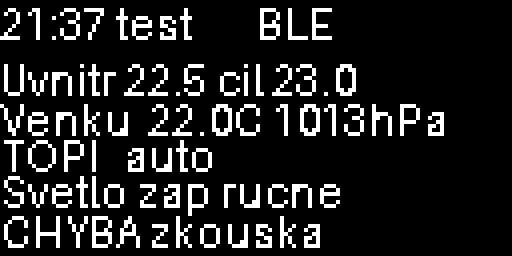
\includegraphics[width=0.55\textwidth]{Figures/displej-zkouska.png}
\caption{Testovací obrazovka zkoušky displej s~rozložením řádků podle ovladače (zvětšeno)}
\label{fig:displej}
\end{figure}

Knihovna luma drží každé vytvořené zařízení v~paměti až do konce programu (asi 320~kB), i~když
jeho inicializace selhala. Ovladač proto zařízení vytvoří až poté, co displej odpoví na zkušební
příkaz \kod{0xAE} (vypnutí displeje~\cite{ssd1306}), a~nejvýš desetkrát za běh programu; potom
zůstane porucha \kod{displej} až do restartu.

\section{Nastavení}
\label{sec:nastaveni}

Nastavení je neměnná datová třída \kod{Nastaveni} se 14 poli; jejich typy, rozsahy, výchozí
hodnoty a~pravidla zápisu jsou v~oddílu~\ref{sec:rozhrani-nastaveni}. Funkce \kod{slouc}
zkontroluje všechny změny a~teprve potom vytvoří nové nastavení, takže při jakékoli chybě
vyhodí \kod{ChybaNastaveni} a~nepoužije se nic.

Po každé platné změně jádro nastavení uloží do souboru \kod{/var/lib/domek/nastaveni.json}
(výpis~\ref{lst:uloz}). Zápis je atomický: JSON se zapíše do pomocného souboru s~příponou
\kod{.tmp}, data se vynutí na disk (\kod{fsync}) a~pomocný soubor se přejmenuje na cílový
funkcí \kod{os.replace}. Nakonec se na disk zapíše i~složka, aby přejmenování přežilo výpadek
proudu. Výpadek tak nenechá rozepsaný soubor: zůstane celý starý, nebo celý nový. Když se
uložení nepovede, změna platí dál a~v~poli \kod{chyby} je \kod{nastaveni}.

\begin{lstlisting}[language=Python, caption={Atomické uložení nastavení (zkráceno z~nastaveni.py)}, label=lst:uloz]
pomocny = cesta + ".tmp"
with open(pomocny, "w", encoding="utf-8") as soubor:
    json.dump(nastaveni.jako_dict(), soubor, indent=2)
    soubor.flush()
    os.fsync(soubor.fileno())   # data musí být na disku dřív než přejmenování
os.replace(pomocny, cesta)
_zapis_slozku_na_disk(slozka or os.curdir)
\end{lstlisting}

Funkce \kod{nacti} soubor při startu načte a~zkontroluje stejnou funkcí \kod{slouc}; chybějící
nebo poškozený soubor nahradí výchozím nastavením. Starší verze programu ukládaly volbu nočního
světla pod klíčem \kod{svetlo_pri_pohybu}. Funkce \kod{nacti} ho převede na nový název
\kod{nocni_svetlo_pri_pohybu}, a~když jsou v~souboru oba klíče, platí nový. Bez převodu by
\kod{slouc} starý klíč odmítl jako neznámý a~zahodil by celý soubor včetně uložené barvy světla.

\section{Server Bluetooth LE}
\label{sec:ble-server}

Třída \kod{BleServer} v~modulu \kod{ble_server.py} vytvoří pomocí knihovny
bluezero~\cite{bluezero} periferii \kod{Termostat} na prvním adaptéru, který BlueZ nabídne,
se dvěma primárními službami: standardní Environmental Sensing Service (ESS) a~vlastní službou
Domek (oddíl~\ref{sec:rozhrani-sluzby}). Metoda \kod{posli_stav} pošle notifikaci Stavu i~hodnot
ESS z~jednoho volání \kod{stav()}, ale jen odebíraným charakteristikám. Zápisy Nastavení
a~Příkazu se zpracují hned v~obsluze zápisu a~server po nich pošle notifikace podle
oddílu~\ref{sec:rozhrani-notifikace}; neplatný zápis zaloguje a~odmítne chybou protokolu ATT
(Attribute Protocol), jak popisuje oddíl~\ref{sec:rozhrani-odmitnuti}. Server také počítá
připojená zařízení a~dokud je nějaké připojené, ukazuje displej \kod{BLE}.

Funkce \kod{_oprav_bluezero} při vytvoření serveru upraví čtyři vlastnosti knihovny bluezero
0.9.1. Čtení respektuje posun (offset), takže klient s~malým MTU složí dlouhou hodnotu po
částech z~téže hodnoty. Čtení ani zápis už nemění vlastnost \kod{Value}, kterou by BlueZ rozeslal
jako nechtěnou notifikaci. Odmítnutá registrace služeb nebo inzerátu, zrušení inzerátu
a~konec démona \kod{bluetoothd} se zalogují a~program skončí, aby ho systemd spustil znovu
a~domek se zaregistroval znovu. Neočekávaná výjimka v~obsluze čtení, zápisu nebo odběru se
zapíše do logu s~výpisem volání, klient dostane chybu a~domek běží dál.

\section{Nasazení}
\label{sec:nasazeni}

Program se na Raspberry Pi nahrává z~PC skriptem PowerShellu \kod{deploy/nahraj.ps1}. Skript
přes SSH (Secure Shell) vytvoří složku \kod{~/domek}, smaže starou složku \kod{~/domek/domek}
(virtuální prostředí \kod{~/domek/venv} nechá), nahraje příkazem \kod{scp} složky \kod{domek}
a~\kod{deploy} se souborem \kod{requirements-pi.txt} a~nakonec službu restartuje příkazem
\kod{systemctl try-restart domek}, takže nová verze platí hned. Mazání odstraní moduly, které
na PC už nejsou, i~složky \kod{__pycache__} patřící rootovi, do kterých by \kod{scp} jako běžný
uživatel nemohl zapsat. Každý vzdálený příkaz se kontroluje a~při chybě skript skončí.

Instalaci na Raspberry Pi dělá skript \kod{deploy/instaluj.sh} spuštěný přes \kod{sudo}.
Spouští se jednou a~potom jen při změně knihoven nebo voleb služby. Postupně:
\begin{enumerate}
  \item zkontroluje volby pro službu funkcí \kod{over_volby} se stejným parserem voleb, jaký má
        program, a~s~neplatnou volbou skončí dřív, než cokoli v~systému změní (odmítne
        i~\kod{--simulace} a~\kod{--help}, se kterými by služba neběžela),
  \item aktualizuje seznam balíčků a~nainstaluje balíčky z~apt (oddíl~\ref{sec:prostredi}),
  \item zapne I\textsuperscript{2}C příkazem \kod{raspi-config nonint do_i2c 0}, ale jen když
        zapnuté není, a~hned potom zavolá \kod{sync} (důvod je v~oddílu~\ref{sec:problemy-hw}),
  \item vytvoří virtuální prostředí a~nainstaluje do něj knihovny z~\kod{requirements-pi.txt},
  \item zapíše jednotku systemd \kod{/etc/systemd/system/domek.service}
        (výpis~\ref{lst:jednotka}), zapne ji pro každý start systému a~službu restartuje.
\end{enumerate}

\begin{lstlisting}[language={}, identifierstyle={}, caption={Jednotka systemd domek.service (cesty pro uživatele admin)}, label=lst:jednotka]
[Unit]
Description=Chytry domek (termostat a cidla ovladane pres Bluetooth LE)
After=bluetooth.service
Wants=bluetooth.service
PartOf=bluetooth.service
StartLimitIntervalSec=0

[Service]
WorkingDirectory=/home/admin/domek
ExecStart=/home/admin/domek/venv/bin/python -m domek
Restart=always
RestartSec=2
Environment=PYTHONUNBUFFERED=1
Environment=PYTHONDONTWRITEBYTECODE=1

[Install]
WantedBy=multi-user.target
\end{lstlisting}

Volby jednotky a~jejich důvody (význam voleb viz~\cite{systemd-unit}):
\begin{description}
  \item[\kod{After=} a~\kod{Wants=bluetooth.service}] domek potřebuje Bluetooth, takže se
        spouští po něm.
  \item[\kod{PartOf=bluetooth.service}] po restartu služby Bluetooth BlueZ registraci domku
        zahodí, proto se zastavení a~restart Bluetooth přenáší i~na domek. Silnější
        \kod{BindsTo=} tu záměrně není: kdyby se služba Bluetooth při startu přeskočila, protože
        se adaptér objevil později, zastavila by domek natrvalo.
  \item[\kod{Restart=always}, \kod{RestartSec=2}] po každém konci programu ho systemd za 2~s
        spustí znovu; tak se léčí i~pozdní start Bluetooth, při kterém se registrace nepovede
        a~program skončí.
  \item[\kod{StartLimitIntervalSec=0}] systemd se po opakovaných pádech nevzdá a~zkouší to dál.
  \item[\kod{PYTHONUNBUFFERED=1}] výpisy jdou do logu (\kod{journalctl -u domek}) hned.
  \item[\kod{PYTHONDONTWRITEBYTECODE=1}] služba běží jako root a~nesmí v~\kod{~/domek/domek}
        vytvářet složky \kod{__pycache__}, které by blokovaly další nahrání.
  \item[bez \kod{User=}] služba běží jako root kvůli registraci v~BlueZ a~nastavení času.
\end{description}
Skript zapisuje do \kod{ExecStart} i~své volby, například \kod{--bme280-adresa 0x77} pro čidlo
na druhé adrese.

\section{Simulace na PC a~zkoušky součástek}
\label{sec:simulace}

Příkaz \kod{python -m domek --simulace} spustí domek na PC se simulovaným hardwarem z~modulu
\kod{hardware/simulace.py}. Čidla mají pevné hodnoty: venku 22~°C, vlhkost 45~\%, tlak
1013,25~hPa a~osvětlení 200~lx; Bluetooth ani skutečný displej v~simulaci nejsou. Simulace běží
ve smyčce po 100~ms: v~každé pauze se zkontroluje pohyb a~po deseti pauzách proběhne krok domku
a~stav se vypíše jako jeden řádek JSON se stejnými klíči jako Stav v~BLE. Kromě
\kod{--simulace} má program tři volby: \kod{--sekund N} (jen v~simulaci, skončí po N krocích,
jinak běží do Ctrl+C), \kod{--nastaveni CESTA} (soubor s~nastavením, výchozí
\kod{/var/lib/domek/nastaveni.json}, v~simulaci \kod{nastaveni-simulace.json})
a~\kod{--bme280-adresa ADRESA} (výchozí \kod{0x76}). Zkrácené volby program odmítá.

Modul \kod{over_soucastky} zkouší na Raspberry Pi každou součástku zvlášť, bez zbytku programu
a~se stejnými ovladači, jaké používá domek, takže ověří i~je. Šest zkoušek (\kod{bme280},
\kod{pir}, \kod{led}, \kod{displej}, \kod{tsl2561} a~\kod{rgb}) a~jejich výsledky na hardwaru
popisuje tabulka~\ref{tab:hw-vysledky}. Před zkouškami \kod{pir}, \kod{led} a~\kod{rgb} se musí
služba zastavit, protože program drží piny GPIO výhradně. U~zkoušek \kod{bme280}
a~\kod{displej} se zastavuje proto, aby se zkouška nemíchala s~tím, co zrovna dělá služba
(souběžné čtení čidla a~kreslení na displej). Zkouška \kod{tsl2561} běží i~při běžící službě. Při
poruše vypíše zkouška řádek \kod{CHYBA:} s~radou, co zkontrolovat.
